\documentclass{rapportECL}
\usepackage{lipsum}
\usepackage{booktabs}
\usepackage{listings}
\usepackage{float}  % in preamble
\usepackage{booktabs}
\usepackage{graphicx}
\usepackage{pgfplots}
\pgfplotsset{compat=1.18}

\title{ECL Report - Template} %File title

\begin{document}

%----------- Report Information ---------

\titre{Perfect Matches} %PDF title
\UE{Data Science Introduction} %Course name
\sujet{Group 1} %Subject name

\enseignant{\Large{Julien \textsc{Velcin} \\
            Erwan \textsc{Versmée}}} %Instructor name

\eleves{\Large{Thomas \textsc{Barand} \\
        Aya \textsc{EL-hajjami}\\
        Oumaima \textsc{LAKLOUCH}}} %Students’ names

%----------- Initialization -------------------

\fairemarges %Display margins
\fairepagedegarde %Create cover page
\tabledematieres %Create table of contents

%------------ Report Body ----------------

\section{Introduction}

L’objectif de ce projet est de concevoir un moteur de recherche pour des articles scientifiques capable d’identifier, pour une requête donnée, les articles les plus proches d’un point de vue sémantique. La requête correspond à un article scientifique, et le système doit retrouver, parmi un ensemble de documents candidats, ceux qui sont réellement pertinents.

Pour chaque requête, un ensemble restreint de documents candidats est fourni, comprenant à la fois des articles pertinents et non pertinents. Le rôle du moteur de recherche est alors d’attribuer un score de similarité à chaque document candidat afin de les classer, en faisant apparaître en priorité les articles pertinents. Ce problème s’inscrit dans le cadre général de la recherche d’information, et plus précisément de la recherche sémantique, où l’enjeu est de dépasser la simple correspondance de mots-clés pour prendre en compte le sens des documents.

Ce projet vise ainsi à comparer différentes approches de représentation des documents et de calcul de similarité, et à évaluer leur capacité à retrouver efficacement les articles pertinents. L’objectif final est d’analyser dans quelle mesure des méthodes modernes de représentation sémantique permettent d’améliorer la qualité des résultats par rapport à des approches plus classiques.

Afin de répondre à cet objectif, le projet est structuré autour des étapes suivantes :
\begin{itemize}
    \item Exploration et analyse des données fournies, incluant le corpus d’articles, les requêtes et les annotations de pertinence ;
    \item Mise en œuvre d’un moteur de recherche de référence basé sur des représentations creuses de type sac-de-mots et TF-IDF ;
    \item Introduction de représentations sémantiques denses à l’aide d’un modèle Sentence-BERT basé sur MiniLM ;
    \item Evaluation comparative des différentes approches à l’aide de métriques standards de la recherche d’information ;
    \item Exploration complémentaire du corpus via des modèles thématiques et l’analyse d’un graphe de citations.
\end{itemize}


\section{Données et Exploration}

Les données utilisées dans ce projet sont fournies sous la forme de trois fichiers principaux. Le fichier \texttt{corpus.jsonl} contient l’ensemble des articles scientifiques constituant la base de recherche. Chaque article est identifié par un identifiant unique et comporte plusieurs champs, notamment le titre, un résumé textuel, des informations de métadonnées (auteurs, année de publication) ainsi que des informations liées aux citations.

Le fichier \texttt{queries.jsonl} contient les requêtes adressées au moteur de recherche. Chaque requête correspond à un article scientifique et ne contient que peu d’informations, principalement un identifiant et un champ textuel correspondant au titre de l’article. Enfin, le fichier \texttt{valid.tsv} fournit les annotations de pertinence sous la forme de triplets (requête, document candidat, score), où le score vaut 1 pour un document pertinent et 0 pour un document non pertinent.

Une exploration initiale des données a permis de mettre en évidence que chaque requête est associée à un ensemble d’environ 25 documents candidats, parmi lesquels seuls cinq sont pertinents. Cette configuration rend le problème particulièrement adapté à une tâche de classement, dans laquelle l’objectif est de faire apparaître les documents pertinents en tête de liste.


\section{Exploration des modèles thématiques}

Dans cette partie exploratoire, nous avons appliqué un modèle de découverte de thématiques latentes pour mieux comprendre la structure sémantique du corpus. L'objectif est d'identifier les grandes thématiques présentes dans les 25\,657 articles et d'évaluer leur distribution, offrant ainsi une perspective complémentaire aux approches de recherche par similarité.

\subsection{Méthodologie : Latent Dirichlet Allocation (LDA)}

Le modèle LDA (\textit{Latent Dirichlet Allocation}) a été utilisé pour extraire automatiquement les thématiques du corpus. Ce modèle probabiliste suppose que chaque document est un mélange de thématiques, et que chaque thématique est une distribution de mots. 

Le prétraitement des textes a été réalisé avec les étapes suivantes : extraction des titres et résumés, vectorisation via \textit{CountVectorizer} avec un vocabulaire limité à 5\,000 termes, et application de filtres fréquentiels (min\_df=5, max\_df=0.7) pour éliminer les mots trop rares ou trop fréquents. Le modèle a été configuré pour identifier 10 thématiques, ce nombre représentant un compromis entre granularité et interprétabilité.

\subsection{Résultats et analyse}

Le modèle a convergé avec une perplexité de 1\,761.80, identifiant 10 thématiques distinctes et interprétables. La Figure~\ref{fig:lda_topics} présente la distribution des documents par thématique dominante ainsi que les mots les plus représentatifs de six thématiques sélectionnées.

\begin{figure}[H]
    \centering
    \begin{minipage}{0.48\textwidth}
        \centering
        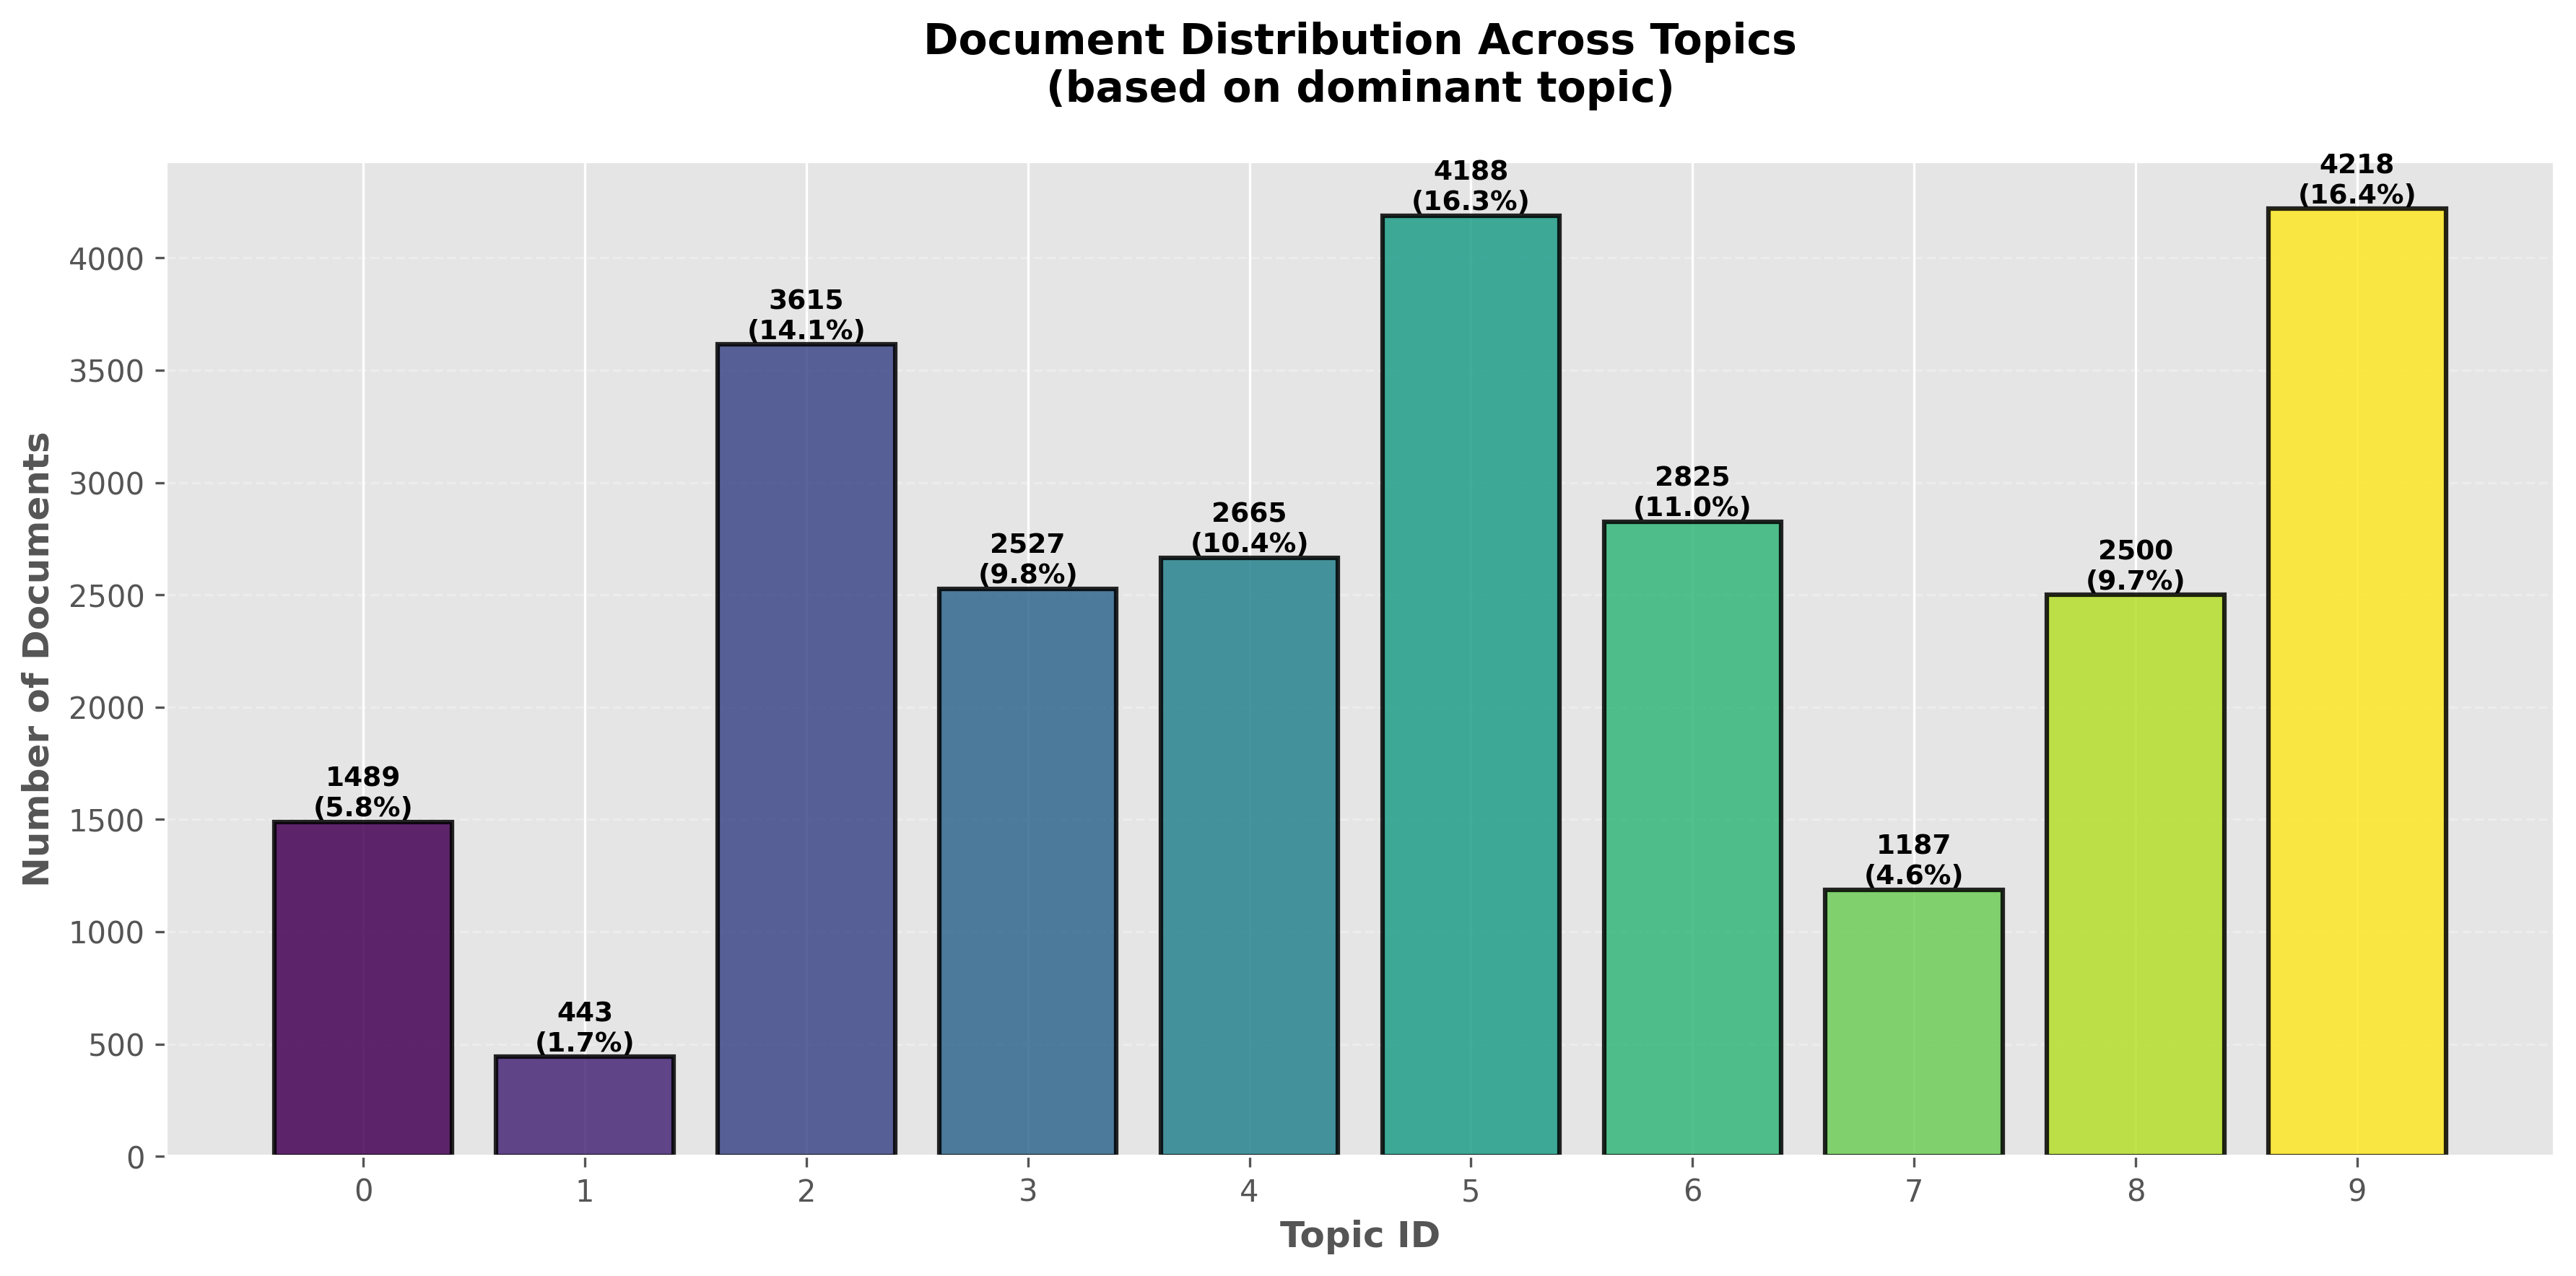
\includegraphics[width=\textwidth]{images/lda_topic_distribution.png}
    \end{minipage}
    \hfill
    \begin{minipage}{0.48\textwidth}
        \centering
        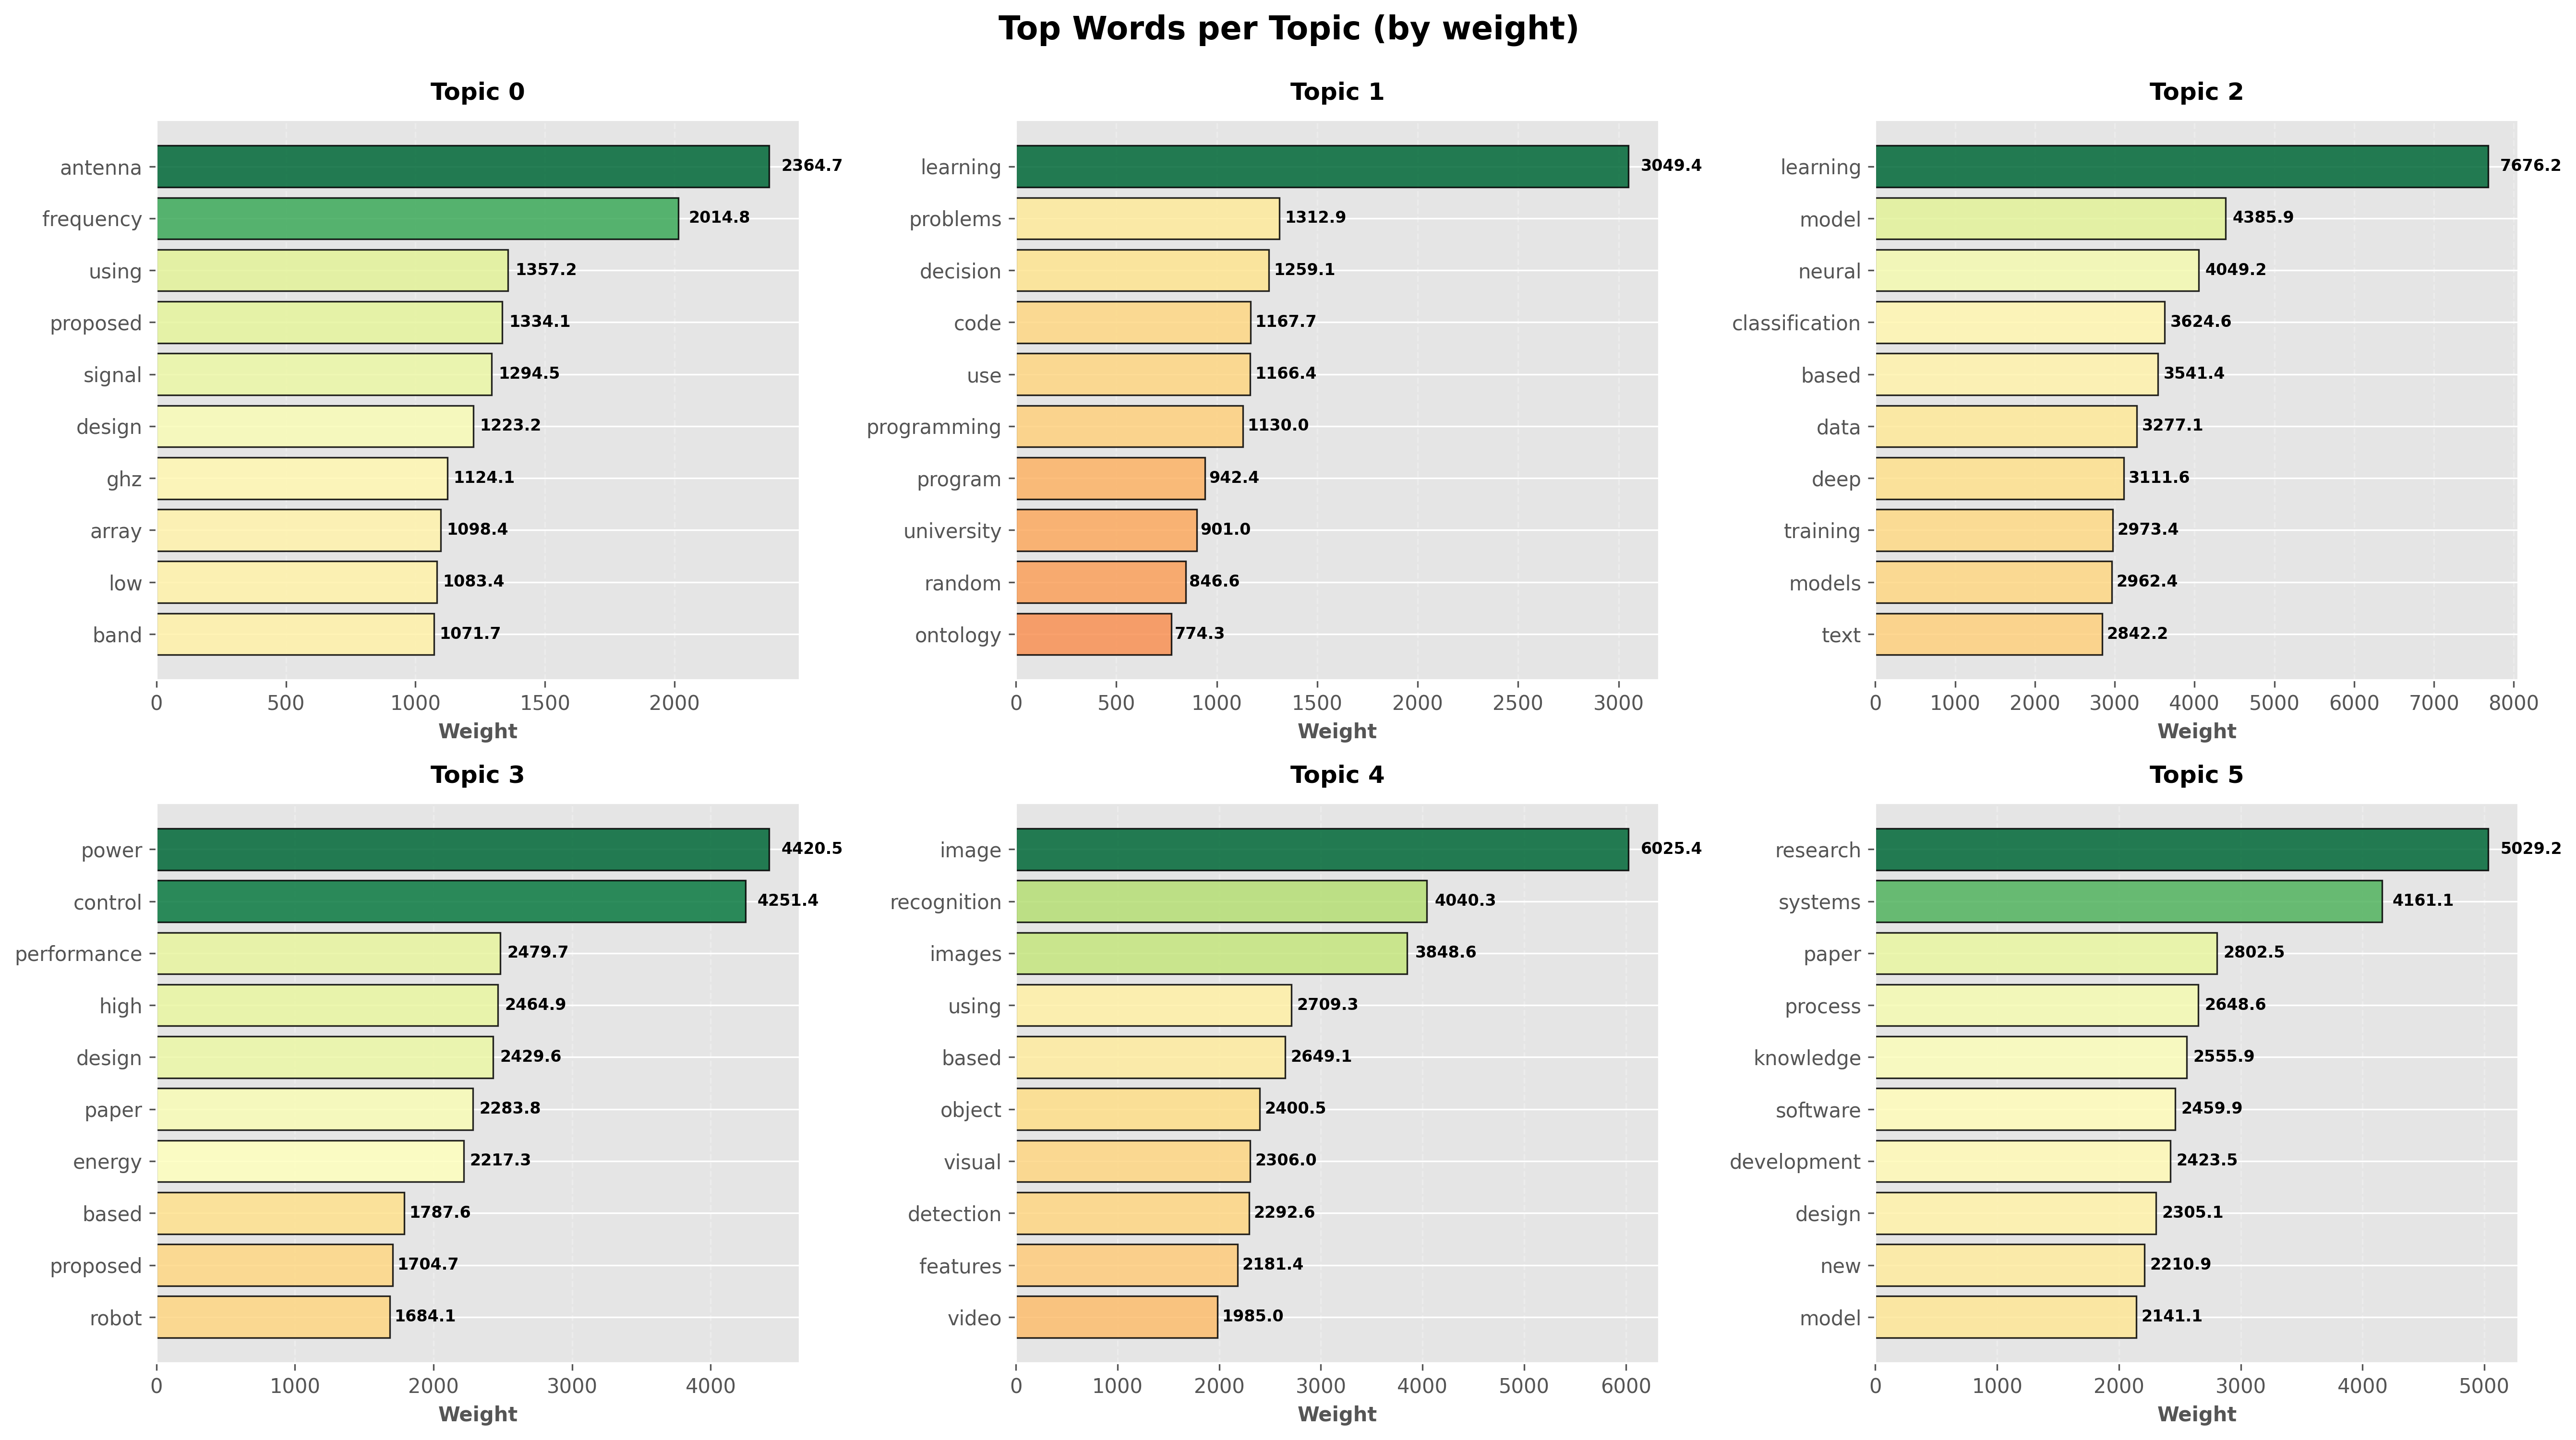
\includegraphics[width=\textwidth]{images/lda_top_words.png}
    \end{minipage}
    \caption{Gauche : Distribution des 25\,657 documents par thématique dominante. Droite : Mots les plus représentatifs pour six thématiques sélectionnées (Topics 0-5).}
    \label{fig:lda_topics}
\end{figure}

L'analyse révèle trois thématiques dominantes : Algorithmes (16.4\%), Systèmes Logiciels (16.3\%) et Machine Learning (14.1\%), qui représentent collectivement près de 47\% du corpus. Les autres thématiques identifiées couvrent des domaines variés tels que la vision par ordinateur (image, recognition, detection), les télécommunications (antenna, frequency, signal), les réseaux et sécurité (network, security, sensor), ainsi que des études médicales (patients, health, study).

Pour mieux visualiser la séparation entre thématiques, une projection t-SNE a été appliquée aux distributions thématiques des documents (Figure~\ref{fig:lda_tsne}). Cette réduction de dimension à 2D permet d'observer la structure de l'espace thématique : les documents d'une même thématique forment des clusters distincts, confirmant la qualité de la séparation thématique identifiée par le LDA.

\begin{figure}[H]
    \centering
    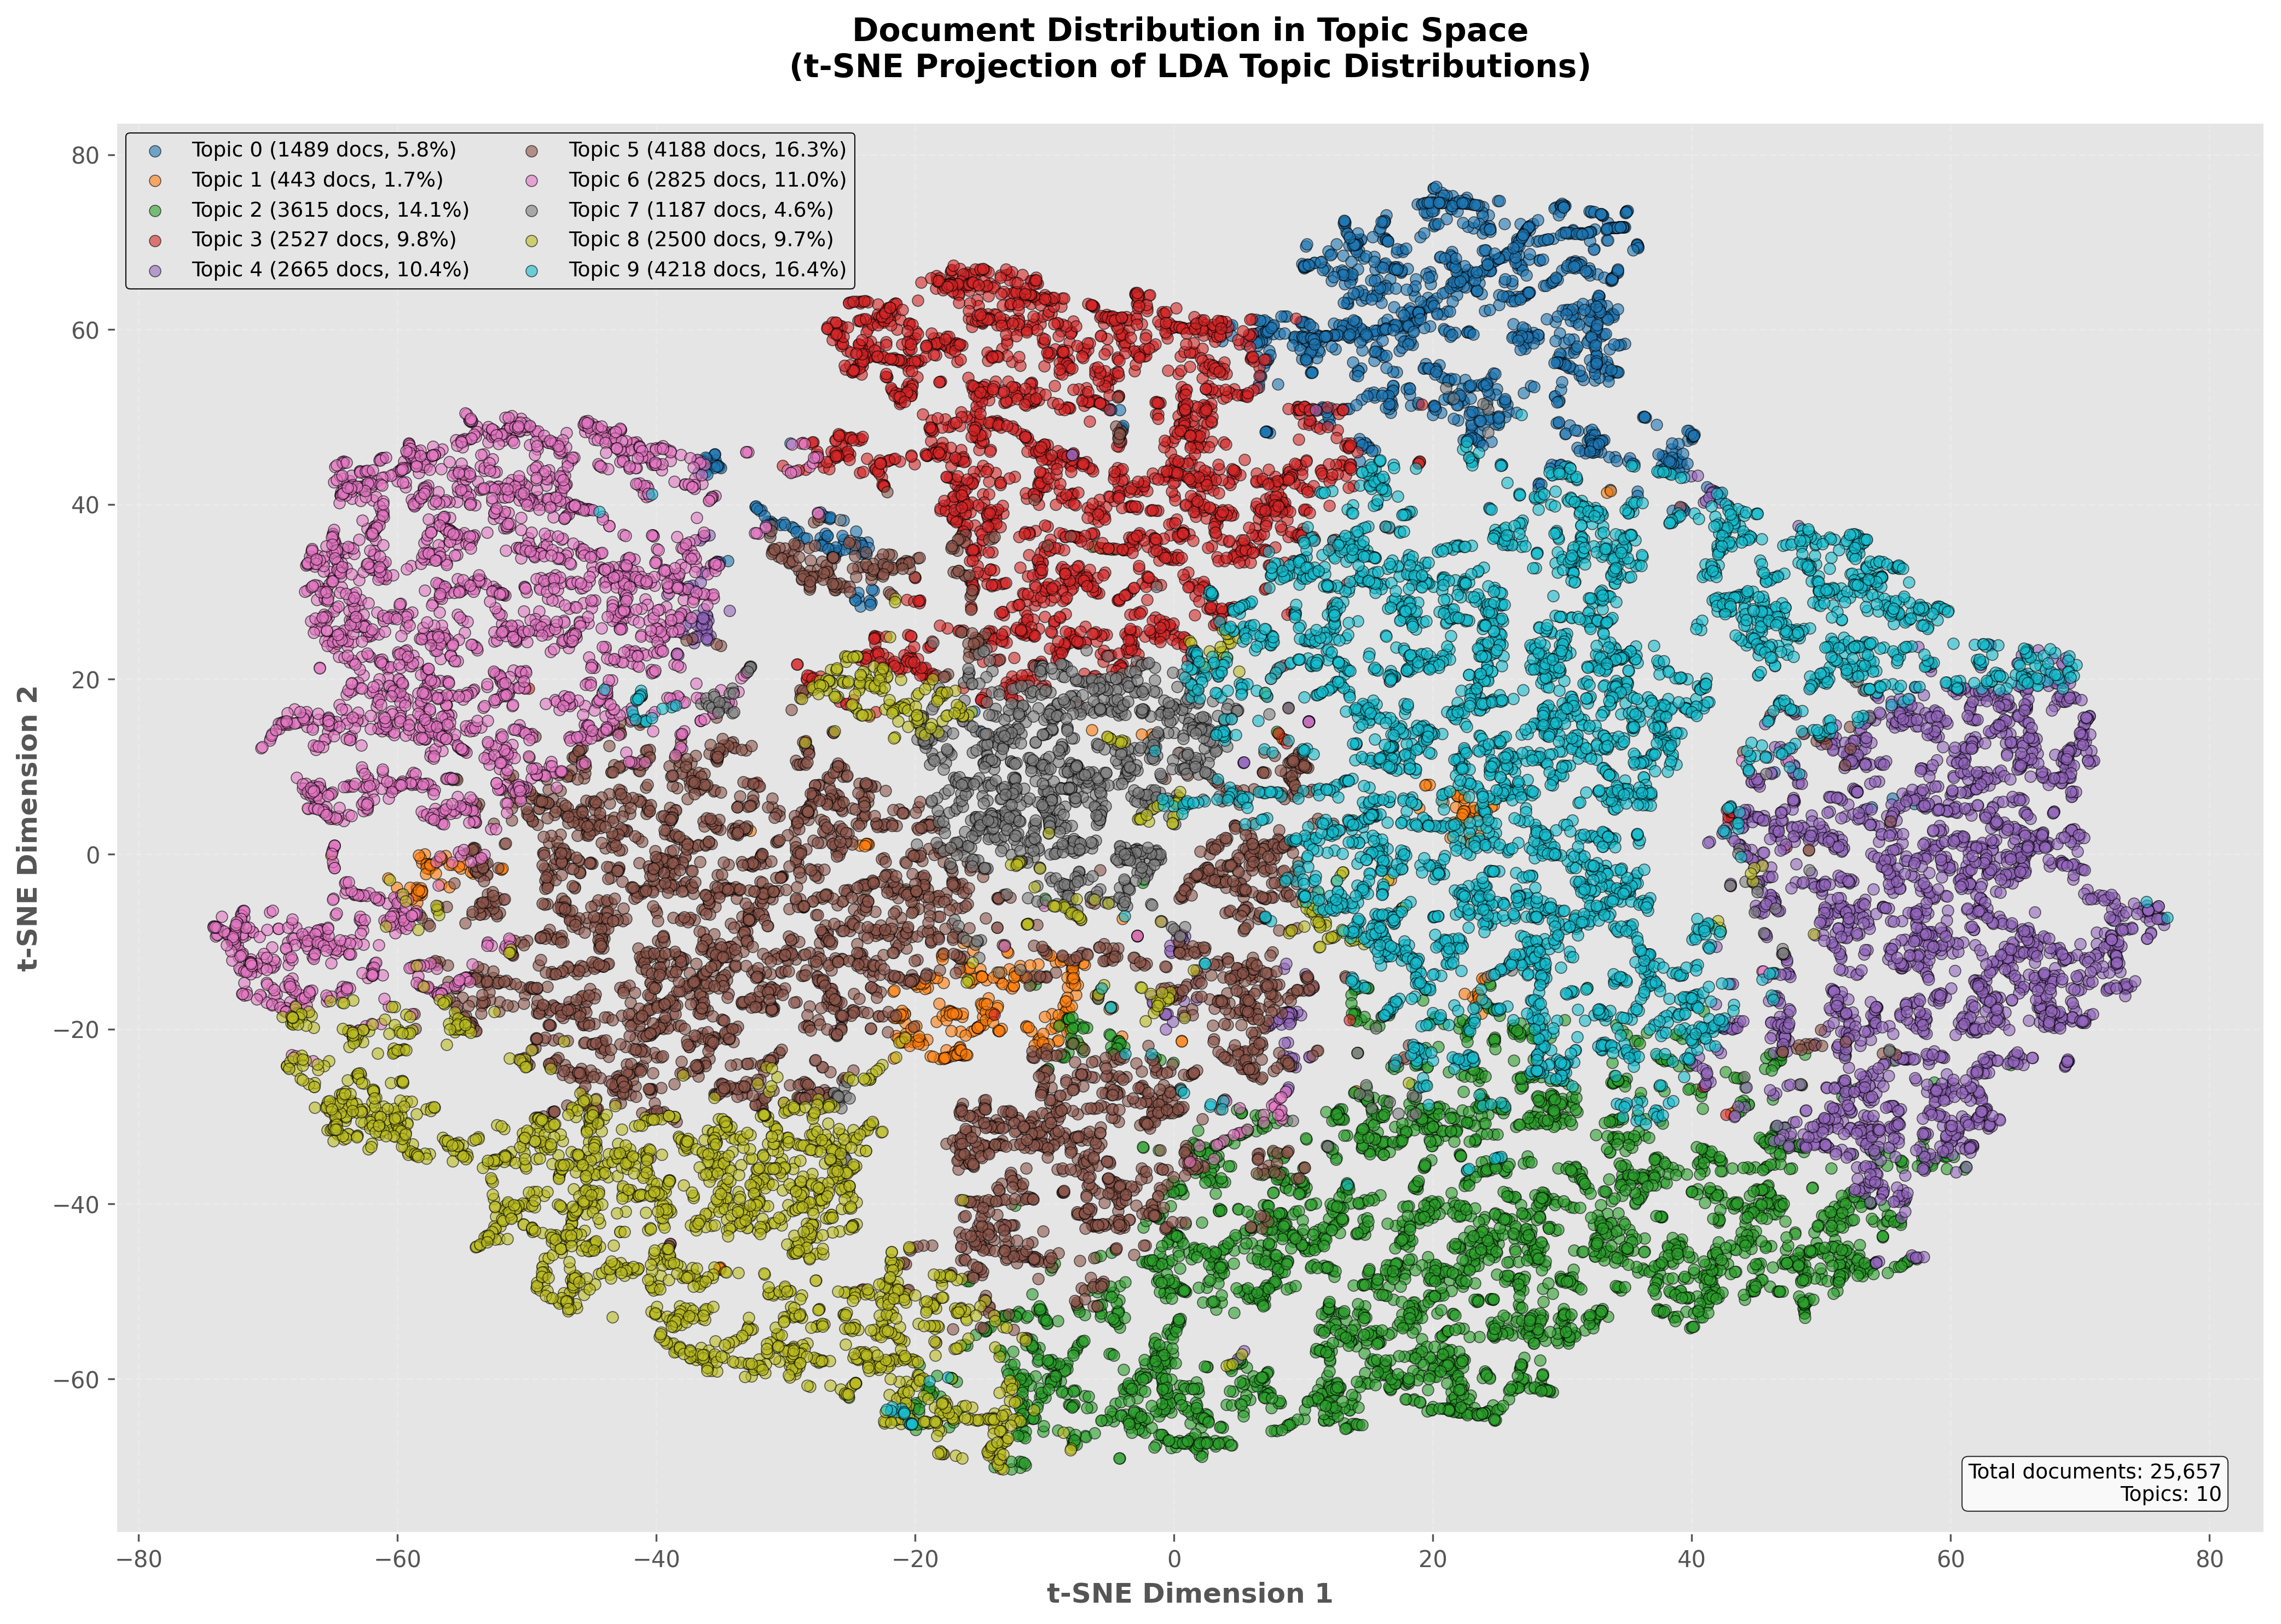
\includegraphics[width=0.85\textwidth]{images/lda_tsne_projection.png}
    \caption{Projection t-SNE des 25\,657 documents dans l'espace thématique. Chaque point représente un document, coloré selon sa thématique dominante. Les clusters visibles confirment la séparation des 10 thématiques identifiées par le LDA.}
    \label{fig:lda_tsne}
\end{figure}

Cette hétérogénéité confirme la diversité du corpus et explique en partie la difficulté de la tâche de recherche : des articles pertinents peuvent appartenir à des domaines thématiques très différents. Bien que cette exploration n'ait pas été intégrée directement dans le moteur de recherche final, elle offre une compréhension précieuse de la structure du corpus et pourrait servir de base à des développements futurs, notamment pour des systèmes de filtrage thématique ou d'enrichissement de features.




\section{Méthodes de représentation et recherche d'information}

L'objectif de cette partie est de trouver les articles, ...

Différentes approches ont été explorées: sparse embeddings, ....

\subsection{Représentations creuses}

La première approche repose sur les représentations creuses de type sac-de-mots, où chaque document est représenté par un vecteur de fréquences de termes. Cette approche ne nécessite aucun apprentissage supervisé et de permet une interprétation directe des résultats mais elle souffre de nombreuses limitations due à sa nature.

\subsubsection{Prétraitement et construction du vocabulaire}

La construction des représentations creuses commence par l'extraction et le nettoyage des textes. Pour les requêtes, les textes extraits sont les titres. Pour le corpus, deux approches ont été envisagées : l'extraction du titre seul, ou du titre et de l'abstract. La recherche basée uniquement sur le titre simplifie le processus tout en produisant, dans ce cas, des résultats équivalents.

La pipeline de prétraitement est la suivante : conversion en minuscules, suppression de la ponctuation, tokenisation et stemming simple. Les mots-outils ("\textit{stop words}") les plus fréquents (37 termes tels que "the", "and", "of") sont supprimés. Un filtrage par fréquence est ensuite appliqué, conservant uniquement les termes apparaissant entre 3 et 350 fois dans le corpus, permettant d'éliminer à la fois les termes trop rares (\textbf{possibles erreurs}) et trop fréquents (\textbf{faible pouvoir discriminant}).

La Figure \ref{fig:vocab_comparison} illustre l'impact de cette décimation sur la distribution du vocabulaire. Le vocabulaire initial de 8\,123 termes est réduit à 2\,671 termes, soit une réduction de 67\%, tout en conservant les termes les plus discriminants pour la tâche de recherche.

\begin{figure}[H]
    \centering
    \begin{minipage}{0.48\textwidth}
        \centering
        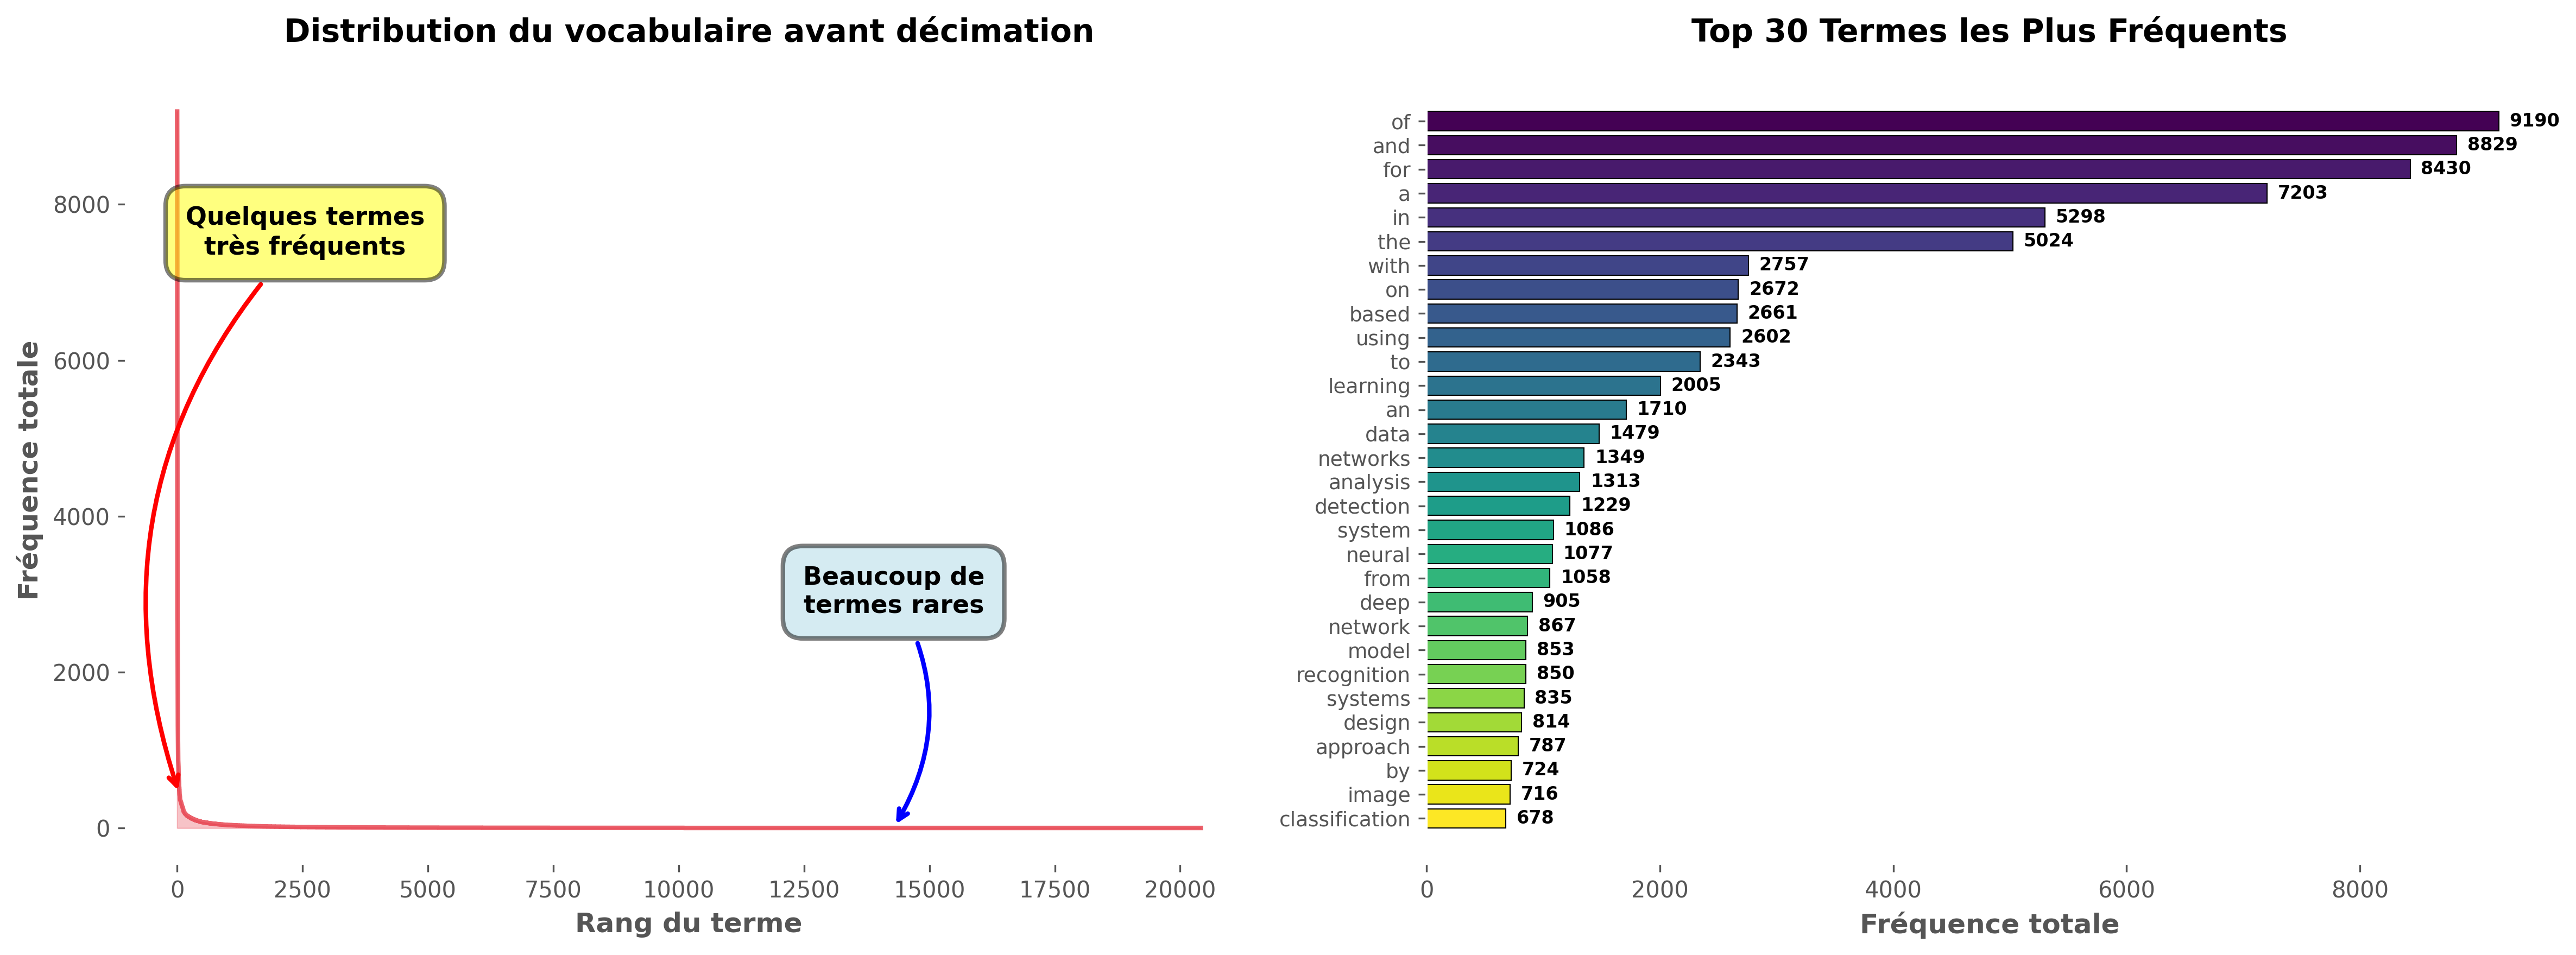
\includegraphics[width=\textwidth]{images/vocab_distribution_before.png}
    \end{minipage}
    \hfill
    \begin{minipage}{0.48\textwidth}
        \centering
        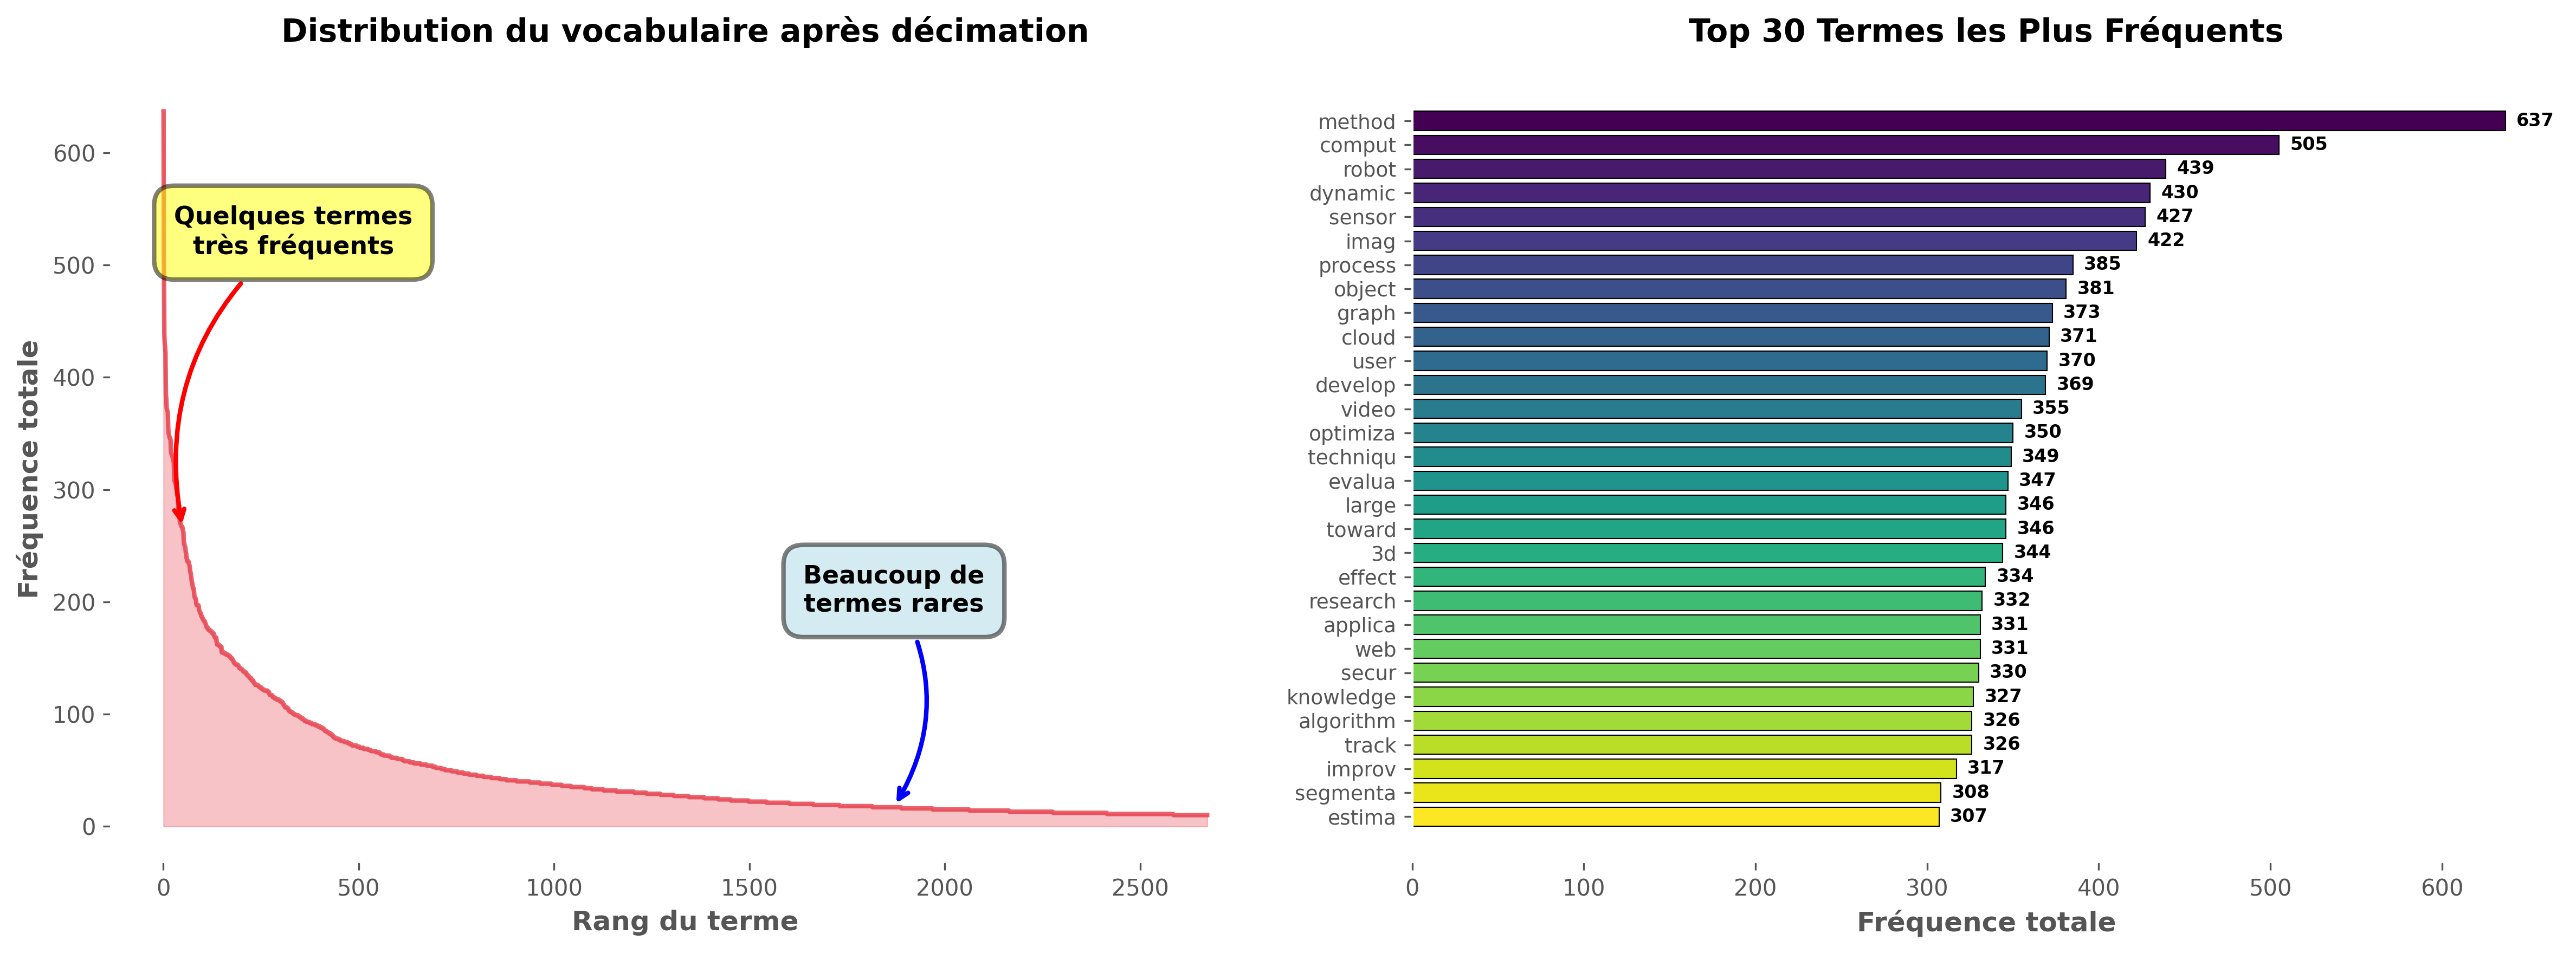
\includegraphics[width=\textwidth]{images/vocab_distribution_after.png}
    \end{minipage}
    \caption{Distribution du vocabulaire avant (gauche) et après (droite) décimation. La distribution suit une loi de puissance caractéristique, avec quelques termes très fréquents et beaucoup de termes rares.}
    \label{fig:vocab_comparison}
\end{figure}

\subsubsection{Méthodes de recherches}

Trois approches creuses ont été implémentées.

\paragraph{Approche baseline : fréquences brutes}
La première approche consiste en un simple comptage des occurrences de chaque terme dans chaque document. Cette méthode, bien que simple, présente une limitation majeure : tous les termes ont un poids identique, ce qui conduit à surpondérer les mots très fréquents au détriment des termes spécifiques plus discriminants.

\paragraph{Pondération TF-IDF}
Une amélioration est apportée par l'utilisation de la pondération TF-IDF (\textit{Term Frequency - Inverse Document Frequency}), qui attribue un poids élevé aux termes fréquents dans un document mais rares dans le corpus global. Cette pondération permet de valoriser les termes discriminants tout en pénalisant les mots trop communs. L'implémentation utilise une normalisation de la fréquence des termes par la longueur du document, combinée à une transformation logarithmique de l'IDF.

\paragraph{Enrichissement par bigrammes}
Une troisième approche consiste à enrichir le vocabulaire en ajoutant des bigrammes, c'est-à-dire des séquences de deux mots consécutifs. Cette extension permet de capturer des expressions multi-mots importantes pour le domaine scientifique (telles que "neural network" ou "machine learning") qui seraient perdues avec des unigrammes seuls. Le vocabulaire résultant combine environ 144\,000 termes pondérés par TF-IDF (unigrammes et bigrammes) (contre 2671 pour les approches précedentes). Bien que cette approche augmente significativement la dimensionnalité, les optimisations liées à la sparsité des vecteurs (95\% de valeurs nulles) permettent de maintenir des temps de calcul raisonnables.

\subsubsection{Calcul de similarité et optimisations}

Pour chaque paire requête-document, la similarité est calculée à l'aide de la \textit{\textbf{similarité cosinus}} entre les vecteurs de représentation. Plusieurs optimisations ont été mises en œuvre pour gérer les 25 millions de comparaisons nécessaires pour le dataset de test (1\,000 requêtes × 25\,657 documents) :

\begin{itemize}
    \item \textbf{Calcul sparse du produit scalaire} : seules les dimensions non-nulles sont traitées, évitant 95\% des multiplications.
    \item \textbf{Pré-calcul des normes} : les normes des vecteurs documents sont calculées une seule fois et réutilisées pour toutes les requêtes.
    \item \textbf{Sauvegarde incrémentale} : les résultats sont écrits progressivement sur disque, permettant une reprise en cas d'interruption.
\end{itemize}

Ces optimisations permettent de traiter l'ensemble du corpus de façon plus efficacement (~10 minutes pour tous le dataset de test sur un CPU standard).

\subsubsection{Résultats et comparaison}

L'évaluation des différentes approches a été réalisée sur l'ensemble de validation et via les soumissions de la compétition kaggle, en utilisant la métrique \textit{\textbf{AUC-ROC}} (\textit{Area Under the ROC Curve}) qui mesure la capacité du système à classer correctement les documents pertinents au-dessus des documents non pertinents en se soustrayant de la dépendance à un seuil.

\begin{table}[H]
\centering
\begin{tabular}{lccc}
\toprule
Méthode & AUC-ROC & Amélioration & Vocabulaire \\
\midrule
Fréquences brutes & 0.6858 & baseline & 2\,671 \\
TF-IDF & 0.7139 & +4.1\% & 2\,671 \\
Bigrammes + TF-IDF & \textbf{0.7260} & \textbf{+5.9\%} & 144\,000 \\
\bottomrule
\end{tabular}
\caption{Comparaison des performances des différentes approches de représentation creuse sur l'ensemble de validation.}
\label{tab:sparse_results}
\end{table}

Les résultats montrent une amélioration progressive des performances à travers les trois approches. Ces résulats montrent aussi la limite de cette méthode qui se repose uniquement sur les mots eux-mêmes et pas sur leur sens ce qui va être exploré par la suite. Les améliorations de TF-IDF et l'enrichissement par bigrammes apporte des gain supplémentaires significatifs confirmant l'importance du traitement fréquentiel des mots et de le capture des expressions multi-mots. La Figure \ref{fig:results} présente la courbe ROC (gauche) et un exemple de résultats de recherche (droite), illustrant la capacité discriminante de l'approche.

\begin{figure}[H]
    \centering
    \begin{minipage}{0.45\textwidth}
        \centering
        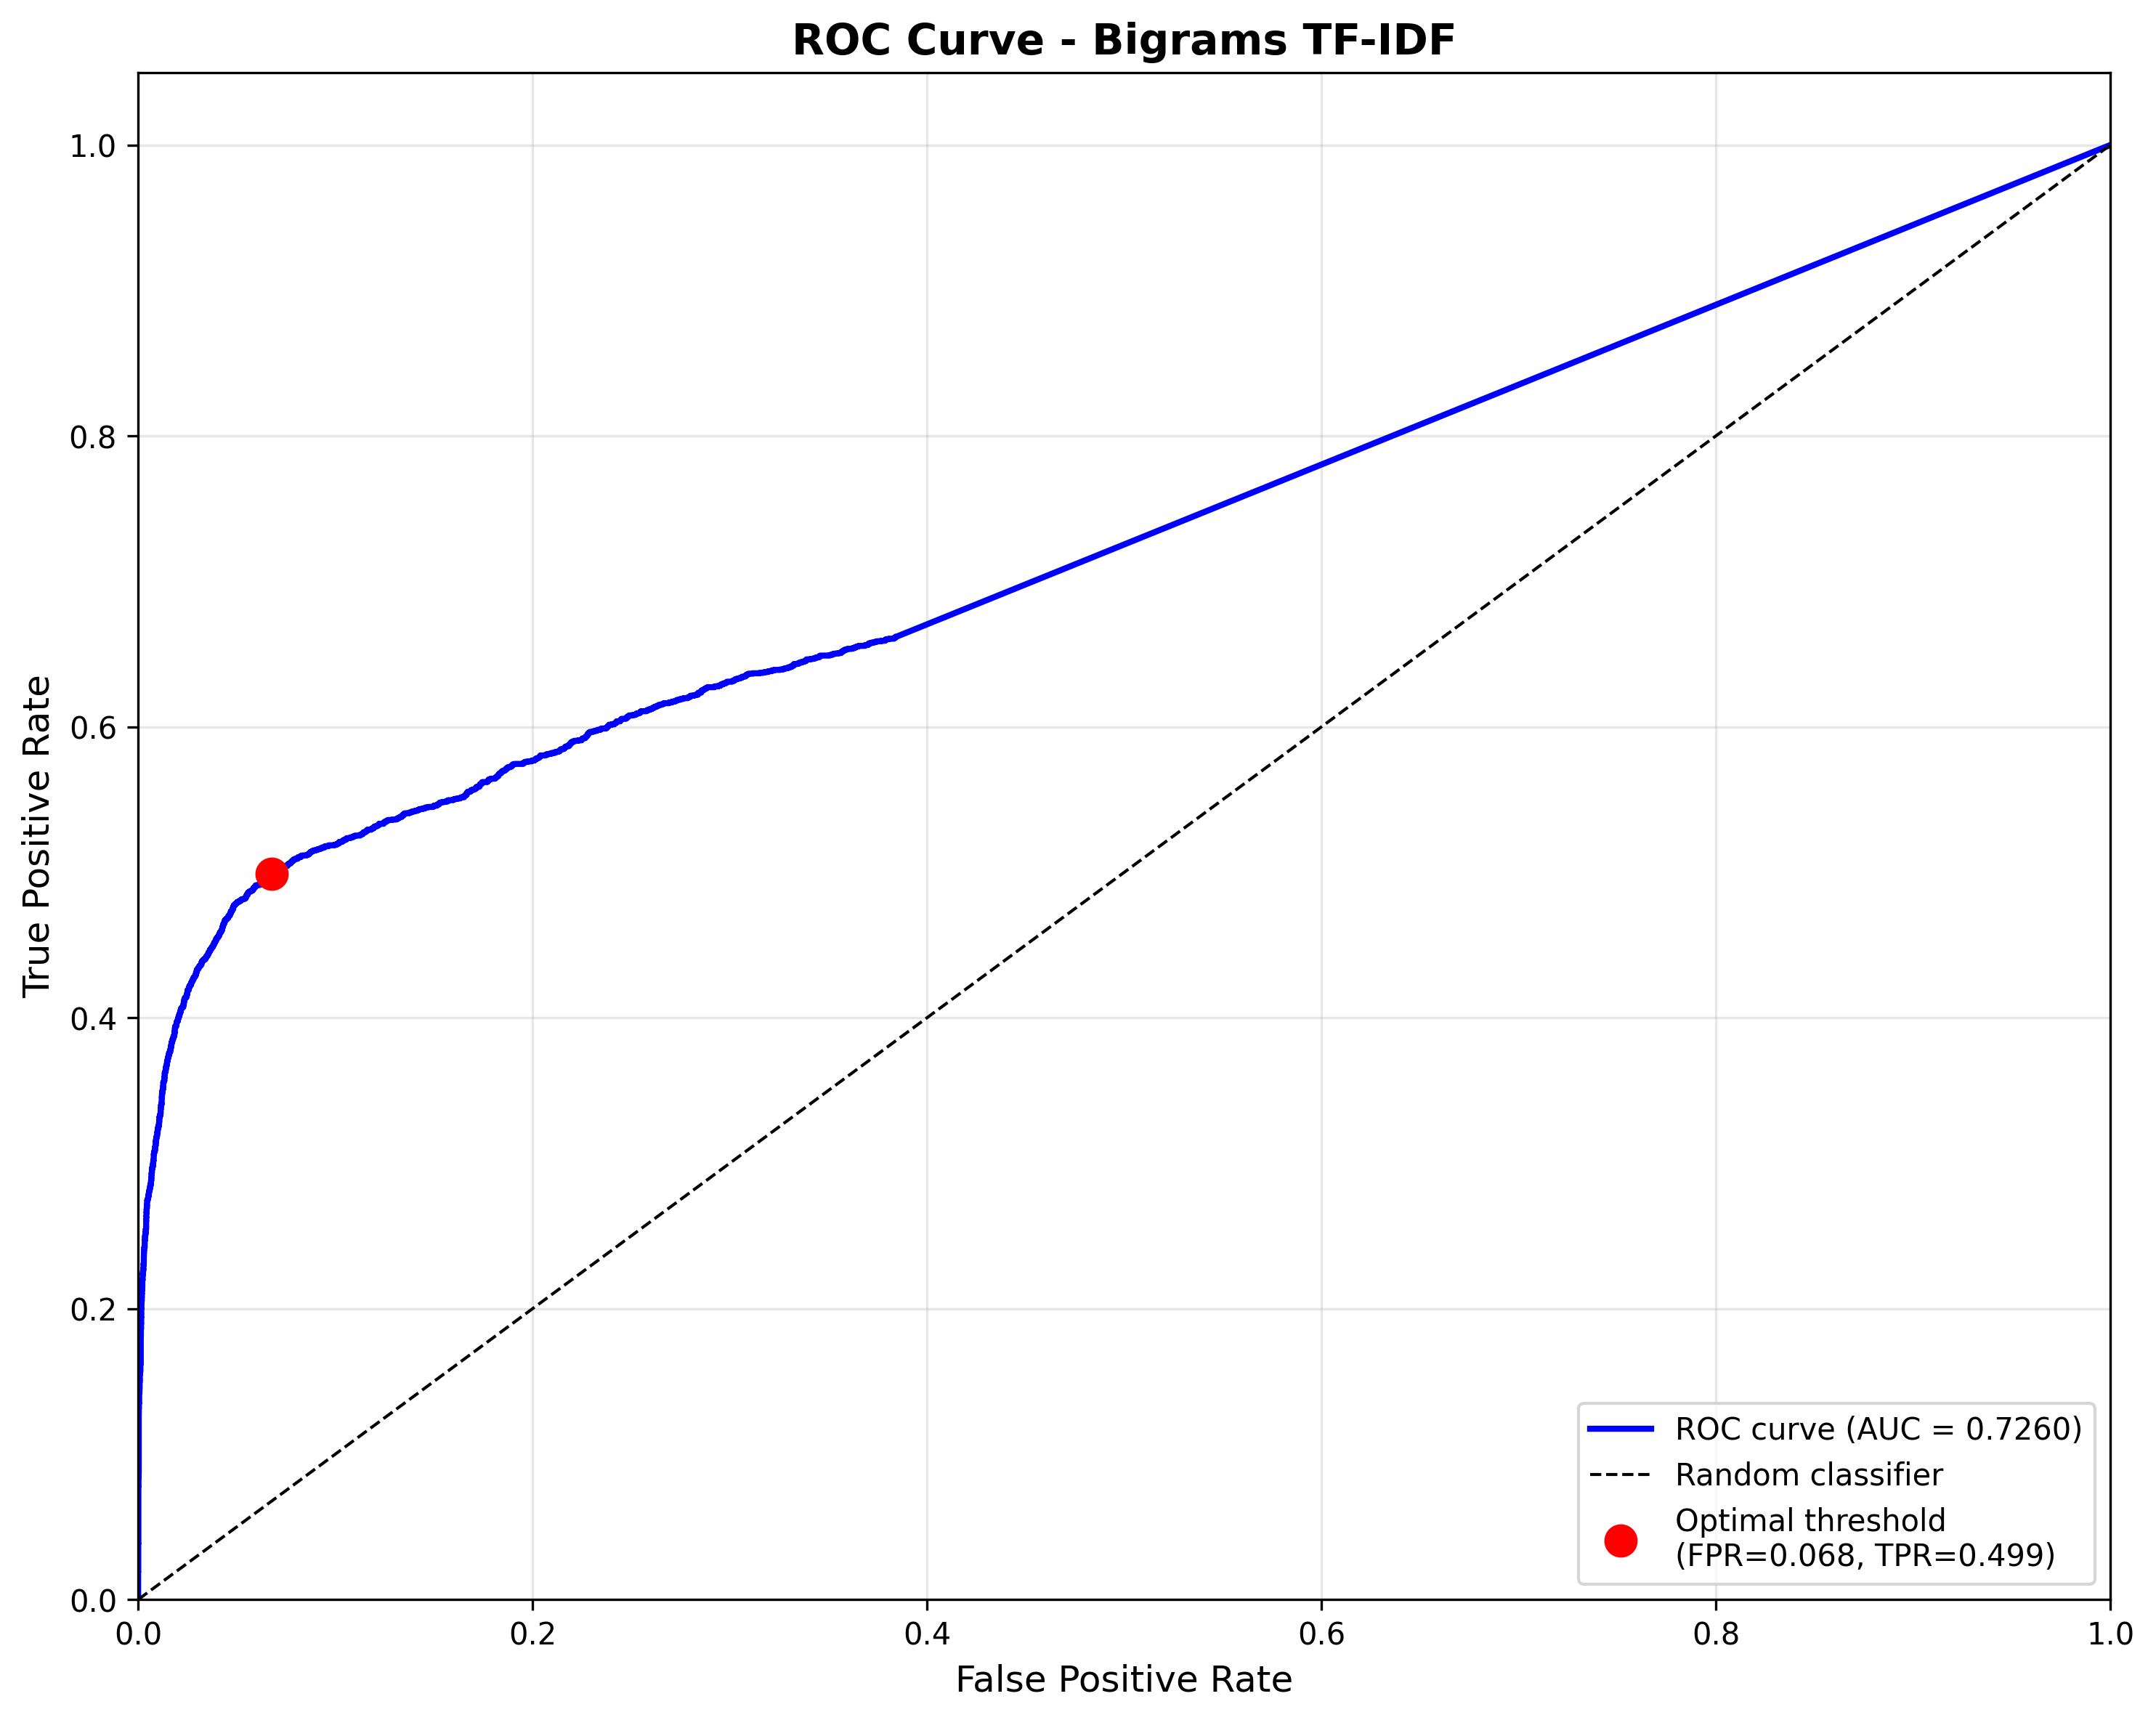
\includegraphics[width=\textwidth]{images/roc_curve_bigram.png}
    \end{minipage}
    \hspace{0.02\textwidth}
    \begin{minipage}{0.45\textwidth}
        \centering
        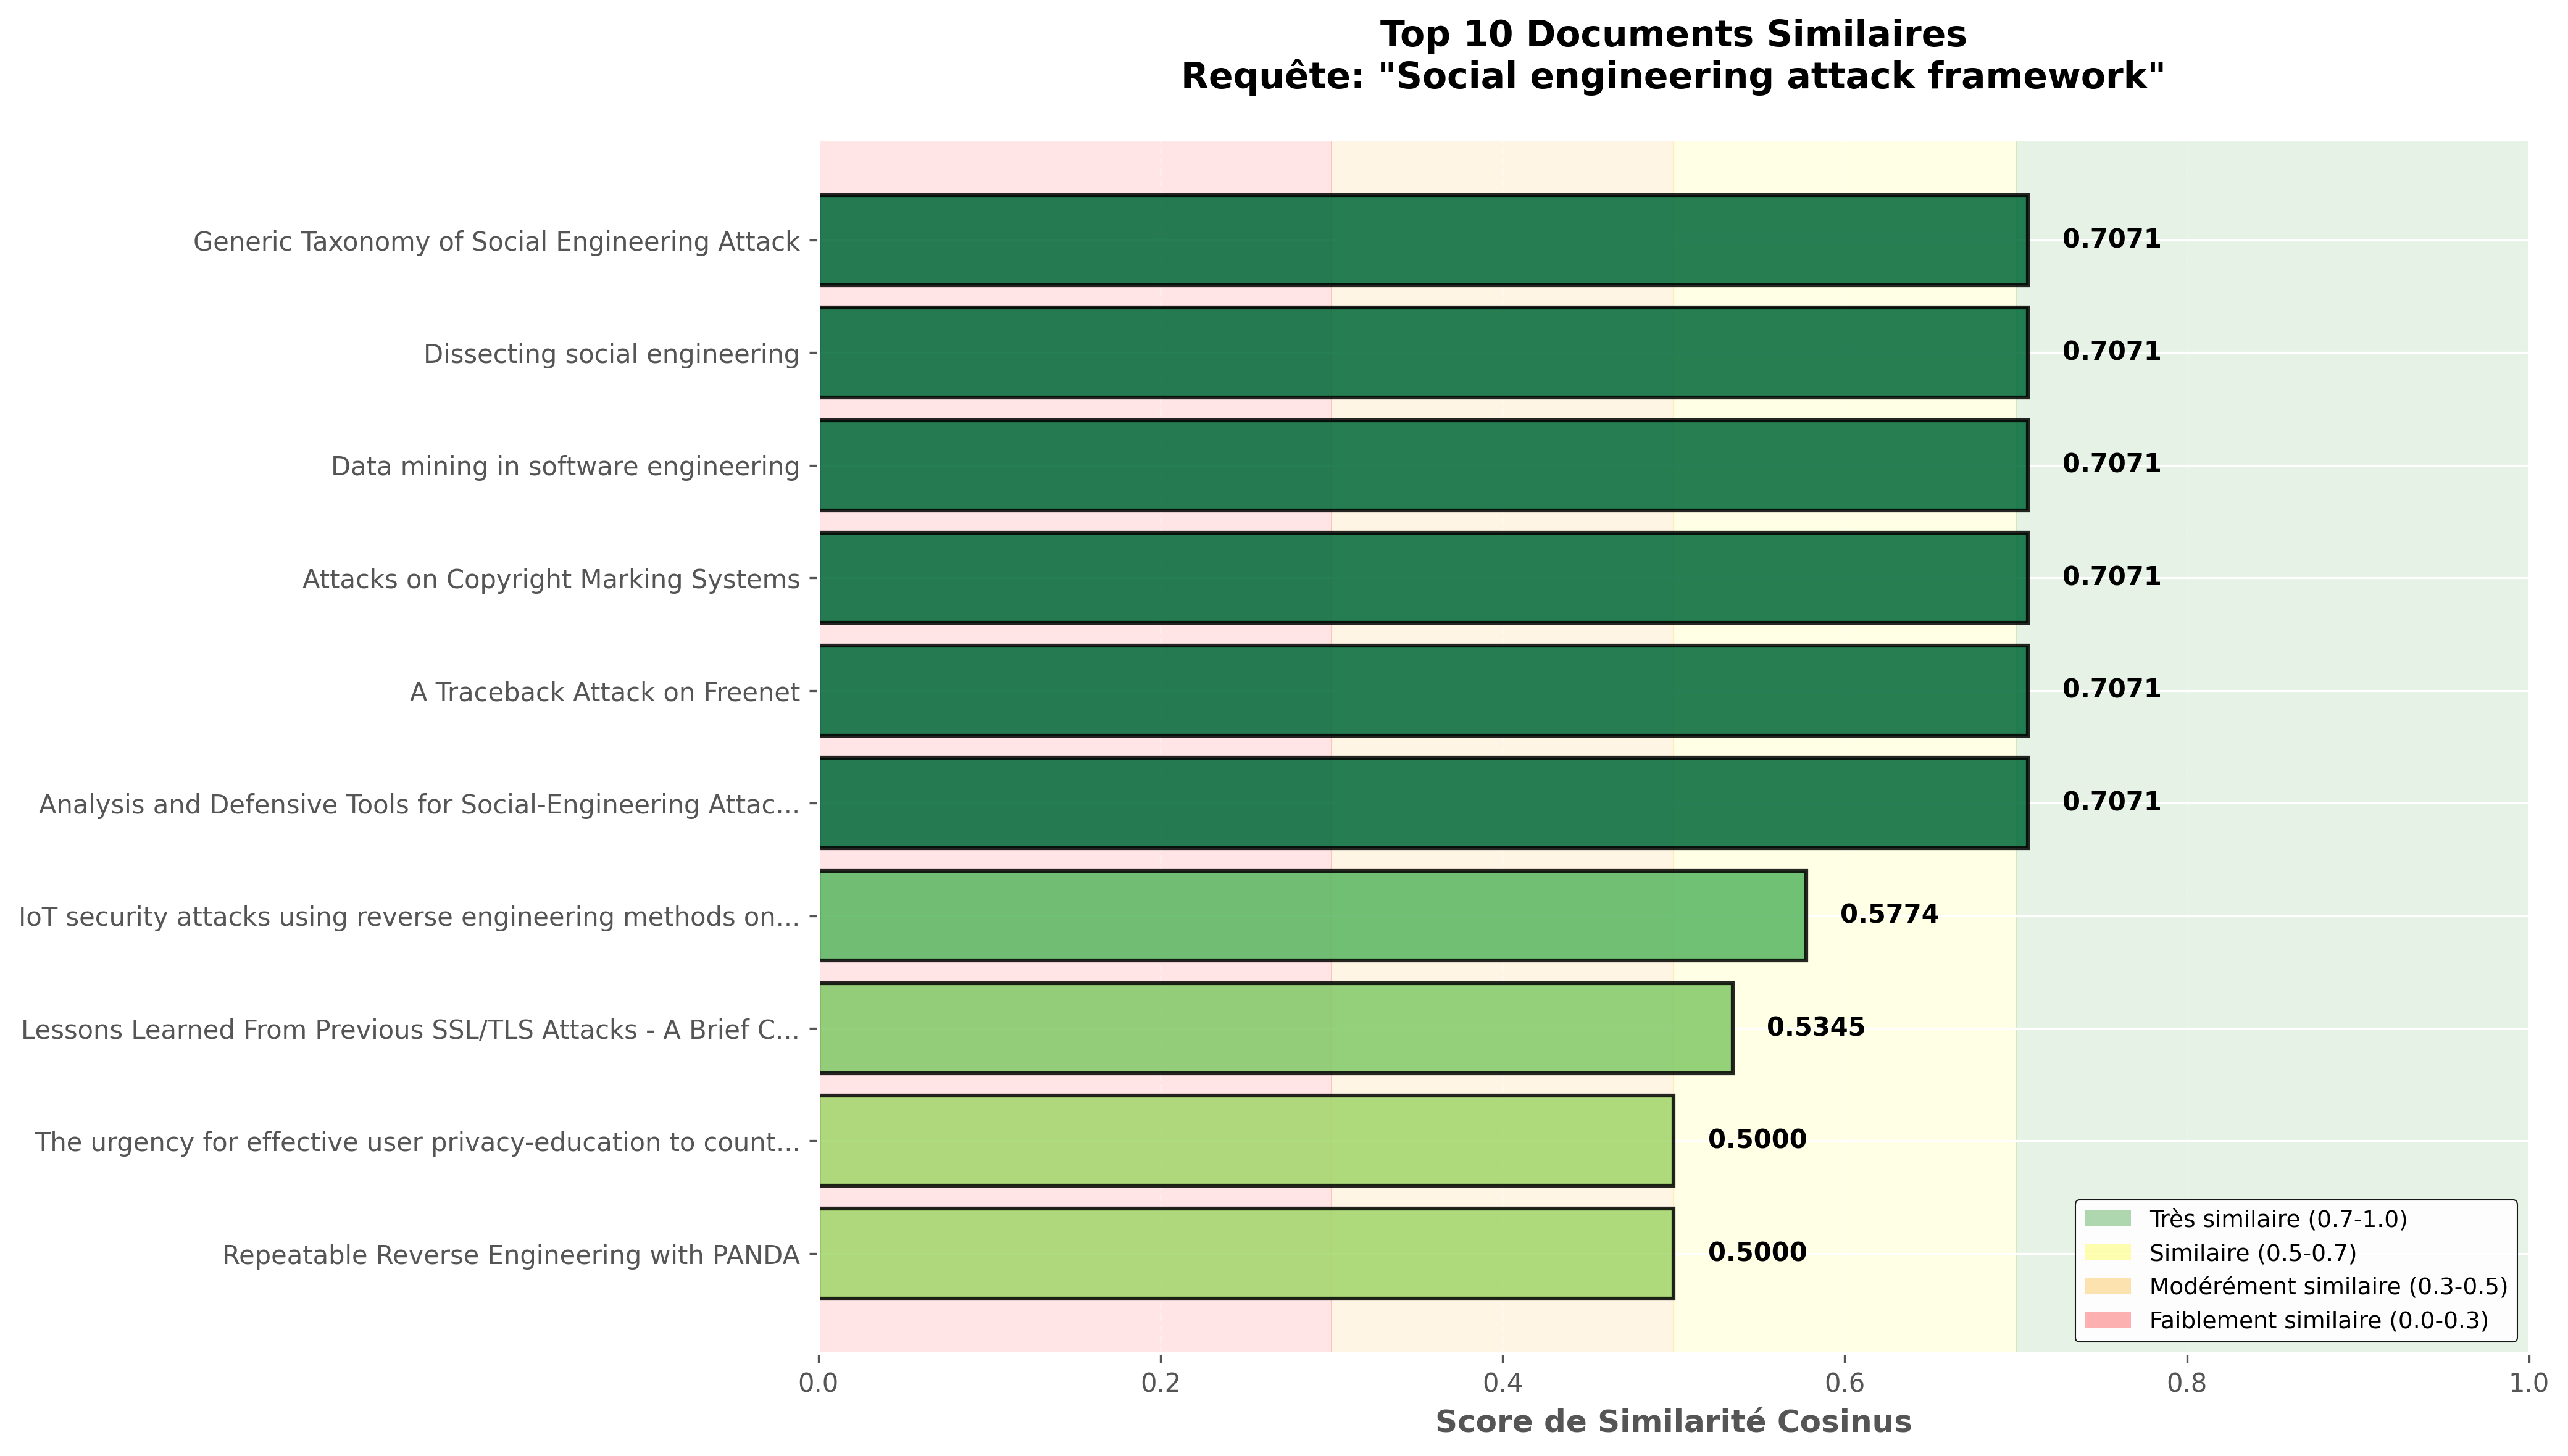
\includegraphics[width=\textwidth]{images/query_similarity_example.png}
    \end{minipage}
    \caption{Gauche : Courbe ROC (AUC = 0.726), le point optimal correspond à un seuil de 0.0081. Droite : Exemple de requête et de résultats ordonnés par similarité.}
    \label{fig:results}
\end{figure}


Ces représentations creuses constituent une base solide pour le système de recherche. Cette approche offre un bon compromis entre performance, simplicité et interprétabilité. Néanmoins, ses limites intrinsèques, notamment l'absence de capture de la sémantique et de la sensibilité aux variations lexicales,  motivent l'exploration de représentations sémantiques denses présentée dans la section suivante.

\subsection{Représentations sémantiques denses avec MiniLM}

Afin de dépasser les limites des représentations creuses, une approche basée sur des représentations denses a été mise en œuvre. Cette approche repose sur l’utilisation d’un modèle de type Sentence-BERT, en particulier le modèle \texttt{all-MiniLM-L6-v2}, qui permet de transformer un texte en un vecteur dense capturant son sens global.

Dans ce projet, seuls les titres des articles ont été encodés, ce choix permettant de réduire les temps de calcul tout en conservant une information sémantique suffisante. Chaque titre est ainsi représenté par un embedding dense de dimension 384. L’ensemble des embeddings du corpus a été calculé une seule fois, puis sauvegardé dans des fichiers au format NumPy afin d’être rechargé rapidement lors des exécutions ultérieures.

La similarité entre une requête et un document est alors calculée à l’aide de la similarité cosinus entre leurs embeddings respectifs. Cette approche permet de comparer les documents sur la base de leur signification plutôt que sur la simple correspondance lexicale, conduisant à une amélioration notable de la qualité des résultats.

\subsection{Graphe de citations et centralité}





\section{Résultats}

L’évaluation du moteur de recherche est réalisée à l’aide des annotations de pertinence fournies dans le fichier \texttt{valid.tsv}. Pour chaque requête, les documents candidats sont classés selon leur score de similarité, et les cinq premiers résultats sont considérés comme les documents prédits pertinents.

Plusieurs métriques classiques de la recherche d’information sont utilisées afin de mesurer les performances globales du système. La précision mesure la proportion de documents correctement identifiés comme pertinents parmi ceux prédits comme tels. Le rappel évalue la capacité du système à retrouver l’ensemble des documents pertinents. La F-mesure combine ces deux indicateurs en une mesure unique. Enfin, l’AUC est calculée à partir des scores continus de similarité et permet d’évaluer la capacité du modèle à distinguer les documents pertinents des documents non pertinents, indépendamment d’un seuil de décision.

Les résultats obtenus montrent que l’approche basée sur les embeddings sémantiques surpasse largement l’approche classique TF-IDF, en particulier en termes de classement des documents pertinents en tête de liste.

\section{Conclusion}







\end{document}
